\documentclass[11pt]{article}
\usepackage[a4paper,margin=24mm]{geometry}
\usepackage[T1]{fontenc}
\usepackage[utf8]{inputenc}
\usepackage{lmodern,microtype}
\usepackage{amsmath,amssymb,amsthm,mathtools}
\usepackage{booktabs,longtable,array,tabularx}
\usepackage{enumitem,xcolor,graphicx}
\usepackage{tikz}
\usetikzlibrary{arrows.meta,positioning}
\usepackage[colorlinks=true,linkcolor=blue!45!black,citecolor=blue!45!black,urlcolor=blue!45!black]{hyperref}
\usepackage{fancyhdr}
\hypersetup{pdftitle={Sparse edge cancellation in unknot recognition},pdfauthor={ProveIt research continuation prepared with ChatGPT}}
\setlength{\headheight}{14pt}
\pagestyle{fancy}
\fancyhf{}
\fancyhead[L]{\small Sparse edge cancellation in unknot recognition}
\fancyhead[R]{\small ProveIt / 12 October 2026}
\fancyfoot[C]{\thepage}
\setlength{\parskip}{4pt}
\setlength{\parindent}{0pt}
\setlist{nosep,leftmargin=*}
\newtheorem{theorem}{Theorem}[section]
\newtheorem{proposition}[theorem]{Proposition}
\newtheorem{lemma}[theorem]{Lemma}
\newtheorem{corollary}[theorem]{Corollary}
\theoremstyle{definition}
\newtheorem{definition}[theorem]{Definition}
\theoremstyle{remark}
\newtheorem{remark}[theorem]{Remark}
\newcommand{\Z}{\mathbb Z}
\newcommand{\Q}{\mathbb Q}
\newcommand{\R}{\mathbb R}
\newcommand{\F}{\mathbb F_2}
\newcommand{\supp}{\operatorname{supp}}
\newcommand{\rank}{\operatorname{rank}}
\newcommand{\spanR}{\operatorname{span}_{\R}}
\newcommand{\poly}{\operatorname{poly}}
\newcommand{\code}[1]{\texttt{#1}}
\newcommand{\kappaV}{\kappa_{\mathrm{v}}}
\newcommand{\cT}{\mathcal T}
\newcommand{\cH}{\mathcal H}
\newcommand{\cC}{\mathcal C}
\title{Sparse edge cancellation in unknot recognition:\\
complete vertex-disc search, explicit obstructions,\\
and compressed boundary interfaces}
\author{A research continuation for Vladimir Reshetnikov's ProveIt project\\
\small Prepared with ChatGPT; working manuscript with exact computational supplements}
\date{12 October 2026}
\begin{document}
\maketitle
\begin{abstract}
We develop a parameter for normal-disc discovery that is independent of the
number of occupied quadrilateral types. For an oriented normal meridian
disc, its geometric edge weights differ from the absolute values of its
signed intersection cocycle only on edges carrying cancellation. On a
one-vertex triangulation with first Betti number one, a meridian whose
cancellation set has size $k$ lies in a known linear space of dimension at
most $k+1$. We prove that all standard vertex meridians with this property
can be recovered by small exact linear systems, without first discovering
their quadrilateral sectors. A sparse-incidence refinement reduces the
number of systems from an elementary $t^{2k+O(1)}$ bound to
$t^{k+O(1)}$ times a factor depending only on $k$. A supported matching
minor and boundary cohomology certify the promised vertex discs in
polynomial bit time, without component-orbit queries. We extend the
discovery theorem to multiple vertices using sign chambers of the cocycle
space.

The new search produces a 47-piece vertex disc on the maintained
eight-tetrahedron example for which the entire primitive coherent family
has genus two. Its cancellation is confined to one interior edge. An
explicit one-dimensional calculation explains this disc, and boundary
layering gives a growing family with the same cancellation parameter.
Conversely, parallel Whitehead curves give finite triangulations of solid
tori on which every meridian has linearly many cancellation edges; this
obstruction allows multiple vertices. We also recover cyclic attachment
data for compressed parallelity bases and distinguish the correct relative
handle replacements for different disc-base interfaces.

The package contains additive code, independent certificate replay,
controlled experiments, and proofs with explicit hypotheses. The
parameterized discovery theorem is unconditional. A logarithmic parameter
bound on a constructively chosen family of knot exteriors is not proved,
so a general quasi-polynomial unknot recognizer is not claimed.
\end{abstract}
\clearpage
{\small\setlength{\parskip}{0pt}\tableofcontents}
\clearpage

\section{Research question and precise scope}
\label{sec:scope}

The maintained project already has substantial exact infrastructure:
normal-coordinate validation, compressed component and disc observers,
independently checked diagram exteriors, coherent cocycle searches,
complete enumeration inside supplied sectors of small dimension,
bounded Pachner searches, and compressed cut geometry. Its most recent
source also contains an all-dimensional source-parallelity construction
with a linear bound on the inherited complementary core
\cite{repo}. The question addressed here is how to discover useful normal
disc vectors without guessing all quadrilateral types or expanding their
possibly enormous integer coordinates.

The 2021 lecture announcement is the motivation for the quasi-polynomial
target \cite{slides}. The July 2026 paper gives a new hierarchy algorithm
and polynomially checkable hierarchy certificates. Its Section 9 explicitly
leaves some step costs unspecified; Proposition 9.1 bounds iterations by
$L(g+1)^L$, and the refined construction controls hierarchy length linearly
\cite{lackenby2026}. These facts do not supply a quasi-polynomial bound for
the maintained implementation. Our results are a separate, parameterized
route to discovery.

\subsection{What is established}

The main results are the following.
\begin{enumerate}
\item A complete exact search for standard vertex meridian discs with
at most $k$ cancellation edges, using spaces of dimension at most $k+1$
on one-vertex, rank-one sources (Theorem~\ref{thm:discovery}).
\item A sparse-incidence enumeration of the determining equations with
an explicit $t^{k+O(1)}$ system-count bound
(Theorem~\ref{thm:incidence}). This is a stronger quantitative statement
than multiplying the number of edge subsets by the number of equation
subsets.
\item An extension with parameter $p+k$, where
$p=\dim H^1(M;\R)+v-1$ is the dimension of the cocycle space
(Theorem~\ref{thm:multivertex}).
\item A new explicit disc and an infinite layered family with cancellation
parameter exactly one; and, in a different class allowing multiple
vertices, a linear lower bound for every meridian.
\item Recovery of the cyclic boundary attachments of compressed
parallelity bases, together with the appropriate relative handle
descriptions for disc bases.
\end{enumerate}

None of the first three statements assumes that a useful quadrilateral
sector has already been supplied. None proves a logarithmic bound on the
new parameter for a universally available source family. The last
distinction is the remaining geometric issue, not a hidden linear-algebra
cost.

\subsection{Meaning of novelty and validation}

Normal edge coordinates, cocycle-dual surfaces, vertex normal surfaces,
and hyperplane-based ray enumeration are established tools. Edge-weight
coordinates are explicitly exposed by Regina \cite{regina}. The local
four-point calculation below is included with proof, rather than claimed
as a new fact about normal surfaces. The proposed contribution is their
combination into a complete cancellation-parameter search, its sparse
enumeration bound, its explicit source families, and the added compressed
interface operator. A literature check and comparison with the pinned
repository found no earlier statement of this particular package of
results. This is not a claim of exhaustive priority verification.

Computations are used to discover examples and test implementations.
Finite tests do not establish asymptotic complexity or replace the proofs.
Likewise, a positive certificate for a supplied triangulation does not
certify that it is the exterior of a particular input diagram. That source
correspondence remains an explicit input to any recognition-level use.

\section{Normal surfaces as compatible four-point metrics}
\label{sec:weights}

Let $\cT$ be a finite triangulation of a compact orientable 3-manifold.
Self-identifications between distinct faces are permitted, but local edge
occurrences and their orientations are retained. Write $t$ for the number
of tetrahedra and $m$ for the number of global edges; always $m\le6t$.
For a normal surface $S$, let
\[
               w_e(S)=|S\cap e|\quad(e\in E(\cT))
\]
be its geometric edge weights. Coordinates count intersections, not signed
intersection numbers and not the sum over repeated local occurrences of
a global edge.

In one tetrahedron label the vertices $0,1,2,3$. Write $t_i$ for the four
triangle coordinates and $q_{ij\mid kl}$ for the quadrilateral separating
$\{i,j\}$ from $\{k,l\}$. This quadrilateral avoids the opposite edges
$ij,kl$. At most one of the three quadrilateral coordinates is positive.
Define the three opposite-edge sums
\[
 s_0=w_{01}+w_{23},\qquad
 s_1=w_{02}+w_{13},\qquad
 s_2=w_{03}+w_{12}.
\]
For every face and every one of its corners put
\[
                 a_i^{jk}(w)=\frac{w_{ij}+w_{ik}-w_{jk}}2.
                 \tag{1}\label{eq:arcs}
\]
These are the numbers of normal arcs cutting off the corresponding corner.

\begin{lemma}[Local reconstruction]
\label{lem:local}
Nonnegative real edge weights in a tetrahedron come from a unique
admissible real standard normal vector if and only if all twelve corner
arc values in \eqref{eq:arcs} are nonnegative and the maximum of
$s_0,s_1,s_2$ is attained at least twice. If all three sums agree, all
quadrilateral coordinates are zero. Otherwise the strictly smaller sum
identifies the avoided pair of edges, and its quadrilateral coordinate is
half the difference between the larger and smaller sums. In either case
\[
                    t_i=\min_{\{j,k\}\subset\{0,1,2,3\}\setminus\{i\}}
                              a_i^{jk}(w).                 \tag{2}\label{eq:triangles}
\]
For integral edge weights, the reconstructed coordinates are integral
exactly when every face has even total edge weight.
\end{lemma}
\begin{proof}
If $q=q_{01\mid23}$ is the occupied type and $T=t_0+t_1+t_2+t_3$,
the edge equations give
\[
                    s_0=T,\qquad s_1=s_2=T+2q.
\]
The other types give the other two permutations of this relation. At a
fixed vertex, two of the corner arc values equal $t_i$, and the third
equals $t_i+q$. This proves necessity and the reconstruction formula.

Conversely suppose, for example, $s_0\le s_1=s_2$. Set
$q=(s_1-s_0)/2$ and use (2) for the triangles. Direct substitution into
the six edge equations gives
\[
 w_{01}=t_0+t_1,\quad w_{23}=t_2+t_3,\quad
 w_{ij}=t_i+t_j+q\quad(ij\notin\{01,23\}).
\]
The assumed corner inequalities give $t_i\ge0$, and the sum inequality
gives $q\ge0$. The formulas determine every coordinate, proving uniqueness.
The all-equal case is the same calculation with $q=0$.

For integer weights, the parity condition makes every number in (1)
an integer. It also makes the differences of opposite sums even: for
example $s_1-s_0$ is even by subtracting the parity equations on the faces
$012$ and $123$. Thus all reconstructed coordinates are integral.
The converse follows because each normal arc contributes two endpoints
to a face.
\end{proof}

The calculation can be pictured as the distance matrix of a tree with
four labelled leaves. The pendant lengths are $t_i$, and the single
internal length is $q$. This picture includes zero lengths and coincident
leaf locations; strict positivity is not required.

\begin{proposition}[Global edge-coordinate reconstruction]
\label{prop:global}
An assignment of nonnegative real weights to the global edges of $\cT$
is an admissible real normal vector exactly when the local conditions of
Lemma~\ref{lem:local} hold in every tetrahedron. Local reconstruction then
gives its unique standard coordinates. If the weights are rational,
clearing the denominators of those coordinates gives a genuine normal
surface.
\end{proposition}
\begin{proof}
On a paired face the three global edge weights are the same on both sides,
with their local labels permuted. Formula (1) therefore gives the same
three normal arc counts. These are precisely the normal matching
equations. Conversely a normal surface restricts to each tetrahedron as
in the lemma. Unique reconstruction on every tetrahedron gives global
uniqueness. Multiplying rational coordinates by a common denominator
preserves all matching, nonnegativity and quadrilateral constraints.
\end{proof}

\subsection{One common set of hyperplanes}

Fix a compatible choice $Q$ of at most one allowed quadrilateral type in
each tetrahedron. The image $\cC_Q$ of its standard normal cone in edge
coordinates is a pointed rational polyhedral cone. The edge map is a
linear isomorphism on this cone and its linear span: express any vector
in the span as a difference of cone vectors and apply local uniqueness.
Its defining
equalities and inequalities have their boundary hyperplanes among:
\begin{enumerate}
\item the $m$ equations $w_e=0$;
\item the three equations $s_i-s_j=0$ per tetrahedron;
\item the twelve equations $2a_i^{jk}(w)=0$ per tetrahedron.
\end{enumerate}
Denote this list by $\cH$, and write
\[
                     H=m+15t\le21t.                       \tag{3}\label{eq:H}
\]
Repeated or identically zero equations may be removed. Each row has
support on at most four global edges, including after identifications;
its coefficients have uniformly bounded absolute value. To describe a
particular $\cC_Q$, one imposes the appropriate equality between the two
larger sums, the inequality for the third sum, and the corner inequalities.
This description explains why searching the common hyperplane list does
not require prior knowledge of $Q$.

\section{Signed intersections and cancellation support}
\label{sec:cancellation}

Give every global edge an orientation. For a cooriented properly embedded
normal surface $S$, let $c_e(S)$ be the algebraic intersection number with
that edge. A face contains oriented normal arcs with cancelling endpoint
signs, so its oriented edge sum is zero. Thus $c(S)$ is an integral
1-cocycle. If an edge has $p_e$ positive and $n_e$ negative intersections,
then
\[
       w_e=p_e+n_e=|p_e-n_e|+2\min(p_e,n_e)=|c_e|+2z_e,
       \qquad z_e\in\Z_{\ge0}.                             \tag{4}\label{eq:defect}
\]

\begin{definition}
The cancellation support of the cooriented surface is
$F(S)=\{e:z_e>0\}$. Its size counts edges with cancellation, not the
number of cancelling pairs. Cancellation multiplicities may be very large.
For a triangulated solid torus, $\kappaV(\cT)$ is the minimum of
$|F(D)|$ over standard vertex normal meridian discs $D$.
\end{definition}

By a standard vertex surface we mean that its coordinate ray is an
extreme ray of the full nonnegative standard matching cone and its
coordinates are primitive integers. For an admissible vector this is
equivalent to extremality in any containing admissible coordinate sector:
such a sector is a coordinate face of the matching cone. The usual
vertex-disc existence theorem makes the set in the definition nonempty
for a triangulated solid torus \cite{hlp}. We keep the word \emph{vertex}
in the parameter because the discovery proof below uses extremality.
It does not show that an arbitrary small-cancellation disc can be replaced
by a vertex disc with equally small cancellation.

\begin{lemma}[One vertex fixes the cocycle]
\label{lem:cocycle}
Suppose $M$ is connected, orientable, and has torus boundary, $\cT$ has
one global vertex, and $b_1(M)=1$. Let $c$ be a primitive
integer generator of its cocycle lattice. An oriented essential disc with
boundary on the torus boundary has intersection cocycle $c$ or $-c$.
Consequently its weight vector satisfies
\[
                w(D)=b+2z,\qquad b=(|c_e|)_{e\in E}.       \tag{5}\label{eq:base}
\]
\end{lemma}
\begin{proof}
All 0-coboundaries vanish when there is one global vertex. The cocycle
lattice is therefore $H^1(M;\Z)$, a free abelian group of rank one.
An essential simple closed curve on a torus is nonseparating. A small
boundary collar therefore supplies a path from one side of the disc to
the other without recrossing it; equivalently the properly embedded disc
is nonseparating. A closed path crossing it once shows that its dual
cohomology class is primitive. Its cocycle is consequently one of the two
generators. Equation (5) now follows from (4).
\end{proof}

The absolute vector $b$ is itself an admissible normal vector in edge
coordinates. On a tetrahedron a cocycle is the difference of four local
heights, so $b_{ij}=|h_i-h_j|$. These are collinear four-point distances
and satisfy Lemma~\ref{lem:local}. The associated surface is the familiar
coherent cocycle-dual surface. It need not be a disc.

\begin{lemma}[The coherent positive support has small rank]
\label{lem:coherent-rank}
Let $C$ be the nonzero coherent surface of an integral cocycle $c$.
The standard matching kernel restricted to its positive support has
dimension at most $p=\dim Z^1(\cT;\R)$. In particular, when $p=1$ and
$c$ is primitive, $C$ is a primitive standard vertex surface and is
connected, although its genus need not be zero.
\end{lemma}
\begin{proof}
Fix an ordering of the original cocycle heights in each tetrahedron.
The supported coordinates are its nonzero successive height gaps: a
triangle at the minimum, the middle quadrilateral, and a triangle at
the maximum. A tied height constrains its corresponding gap to zero.
For any vector $y$ in the supported matching kernel, regard these
coordinates as formal height gaps. On each local oriented edge the
formal difference equals $\operatorname{sign}(c_e)w_e(y)$, with the
local-to-global edge orientation included. This identity is linear and
does not require $y$ to be nonnegative. If $c_e=0$, all supported normal
types avoid that edge, so $w_e(y)=0$.

Matching makes these edge weights agree at all occurrences of a global
edge. The vector $a_e=\operatorname{sign}(c_e)w_e(y)$ is consequently
a global cocycle. The map $y\mapsto a$ is injective: zero $a$ implies
zero weights, and the edge map is injective on the fixed quadrilateral
support. The dimension bound follows. If $p=1$, the nonzero vector $C$
forces dimension one. A common coordinate divisor of $C$ divides every
weight $|c_e|$, so primitive $c$ makes $C$ primitive. The primitive-ray
component argument of Proposition~\ref{prop:vertex-gate} proves
connectedness.
\end{proof}

\subsection{Computing the primitive generator}

Build the integral face matrix $A$, using one signed equation per global
triangular face and summing repeated edge occurrences. Rank-one nullspace
computation and division by the coordinate gcd produce $c$. The one-vertex
and rank-one hypotheses are checked, not inferred from a filename. Each
row of $A$ has sum of absolute coefficients at most three. Cofactors of
an independent $(m-1)$-row submatrix therefore give a generator with
\[
                    \max_e|c_e|\le3^{m-1}.                \tag{6}\label{eq:cbound}
\]
Hadamard's inequality proves this bound, and primitive division only
decreases it. Exact computation has polynomial bit complexity. In
particular, exponential geometric weights do not entail exponential
input length for this stage.

\section{Complete discovery from low-dimensional weight spaces}
\label{sec:flat-search}

For an edge subset $F$ define
\[
       W_F=\spanR\bigl(\{b\}\cup\{\mathbf e_f:f\in F\}\bigr),
       \qquad d_F=\dim W_F\le |F|+1.                     \tag{7}\label{eq:WF}
\]
Here $\mathbf e_f$ is the coordinate vector of edge $f$. We deliberately
search the whole space $W_F$. Requiring a nonnegative cancellation vector
would make a smaller search, but is unnecessary for soundness: every
returned candidate is reconstructed and topologically checked. In
particular, membership in $W_F$ alone is not an orientation certificate.

\begin{lemma}[Determining an extreme ray by active equations]
\label{lem:active}
Let $W\subset\R^m$ be a $d$-dimensional linear space and let $w\ne0$
generate an extreme ray of a sector cone $\cC_Q$. If $w\in W$, then some
$d-1$ equations from $\cH$, restricted to $W$, are independent and have
common kernel $\R w$ in $W$.
\end{lemma}
\begin{proof}
The ray stays extreme in $\cC_Q\cap W$: a nonproportional nonnegative
decomposition there would also be a decomposition in $\cC_Q$.
Consider all defining equalities and all inequalities active at $w$.
If their common kernel in $W$ had dimension greater than one, choose a
direction $u$ not parallel to $w$ in that kernel. For sufficiently small
$\varepsilon>0$, both $w+\varepsilon u$ and $w-\varepsilon u$ satisfy
every inactive strict inequality as well as the active equations. They
give a nonproportional decomposition of $2w$, a contradiction. Thus the
active kernel is precisely the line $\R w$. Select an independent
$(d-1)$-row subset. Every selected hyperplane belongs to $\cH$ by (3).
The argument includes sectors and intersections that are not full
dimensional.
\end{proof}

\begin{theorem}[Complete cancellation-supported vertex-disc discovery]
\label{thm:discovery}
For a supplied finite triangulation of a compact connected orientable
3-manifold with exactly one torus boundary, one global vertex and $b_1=1$,
there is a
deterministic exact algorithm that finds an essential disc whenever a
standard vertex essential disc has at most $k$ cancellation edges.
The algorithm makes at most
\[
       \sum_{\substack{F\subseteq E\\|F|\le\min(k,m)}}\binom H{d_F-1}
       \ \le\ \sum_{j=0}^{\min(k,m)}\binom mj\binom Hj     \tag{8}\label{eq:basic-count}
\]
small homogeneous linear-system attempts.
Each candidate has polynomially bounded encoded length and is checked
in polynomial bit time. Its overall bit cost is $t^{O(k+1)}$.
If the input is only known to satisfy the source hypotheses, exhaustion
of a smaller $k$ is inconclusive for unknot recognition.
\end{theorem}
\begin{proof}
For every $F$ with $|F|\le k$, compute a basis of $W_F$. Enumerate all
$(d_F-1)$-subsets of $\cH$ and retain those of restricted rank $d_F-1$.
Find the one-dimensional rational kernel, test its two directions for
nonnegativity, and apply Lemma~\ref{lem:local} on every tetrahedron.
Clear denominators in the reconstructed standard coordinates, divide by
their gcd, and apply the polynomial vertex-disc gate of
Proposition~\ref{prop:vertex-gate}. The zero-dimensional case contributes
no ray; a
one-dimensional space needs the empty equation subset.

If $D$ is a promised vertex disc, take its cancellation set $F$. Equations
(5) and (7) put its edge ray in $W_F$. The edge isomorphism preserves its
extremality. Lemma~\ref{lem:active} ensures that one enumerated system
recovers exactly this ray. Primitive normalization then recovers $D$.
The tests cannot manufacture a positive result: they verify genuine
normal coordinates and essential disc topology in the supplied manifold.

The bound counts all systems before pruning or duplicate removal. Exact
linear algebra, reconstruction and the vertex-disc gate are polynomial
in the source and coordinate bit lengths. The bit estimate below makes
these lengths polynomial in $t,k$ and the size of $c$. This proves the
stated parameterized bound without an assumption about the run time of
the repository's present interval-orbit engine.
\end{proof}

\begin{remark}[The displayed count]
The second inequality in (8) is used for $j\le H/2$, which includes the
relevant range $j\le m\le6t$ since $H\ge m+15t$. Then
$d_F-1\le j$ and the binomial coefficients are increasing on that range.
Zero hyperplanes can be left on the list for this upper bound.
\end{remark}

\subsection{Encoded size and verification cost}

Let $B$ bound the bit length of $b_e$ and of the source indices. A basis of
$W_F$ can be selected from $b$ and the coordinate vectors. Restricted
hyperplane coefficients have $O(B+1)$ bits. For a $d$-column system,
cofactor bounds give a null vector whose coordinates have
\[
                         O(d(B+\log(d+1)))                 \tag{9}\label{eq:bits}
\]
bits. Multiplication by the weight-space basis and the half-integer local
reconstruction preserve a polynomial bound. The produced standard
coordinates may describe exponentially many discs, but their binary
encoding and all verification inputs remain polynomial in $t,k,B$.
No estimate is measured in the expanded piece count.

\subsection{A polynomial gate for the promised vertex discs}

There is a useful way to avoid a stronger-than-needed topology subroutine.
Let $M_{\!N}$ be the standard normal matching matrix, and for a nonzero
integral admissible vector $x$ let $J=\supp x$. Its submatrix
$M_{\!N,J}$ retains exactly the positive coordinate columns.

\begin{proposition}[Rank and boundary parity certify a vertex disc]
\label{prop:vertex-gate}
Suppose $\partial M$ is a torus. A primitive nonzero integral admissible
normal vector $x$ is an essential disc if all three tests hold:
\[
 \dim\ker M_{\!N,J}=1,\qquad \chi(x)=1,\qquad
 [\beta(x)]\ne0\ \text{in }H^1(\partial M;\F),
\]
where $\beta(x)_e=w_e(x)\bmod2$ on boundary edges. Every primitive
standard vertex meridian passes these tests. All tests, including
admissibility, primitivity and the boundary coboundary quotient, have
polynomial bit complexity in the encoded source and $x$.
\end{proposition}
\begin{proof}
The nullity test says exactly that the positive support of $x$ spans a
ray of the standard matching cone. If the surface were disconnected,
each component would have an integral normal vector $y_i=\lambda_i x$
with $\lambda_i>0$ and $\sum_i\lambda_i=1$. Since $\gcd(x)=1$, there
are integers $a_j$ with $\sum_j a_jx_j=1$. Thus
$\lambda_i=\sum_j a_j(y_i)_j$ is an integer. There can be only one
component.

On every boundary face, the sum of the three intersection parities is
zero: each normal arc has two endpoints. Hence $\beta$ is a cocycle.
It is the mod-two Poincar\'e dual of the boundary curve system, because
its evaluation on a transverse edge counts precisely those intersections.
The nonzero class implies that the connected surface has nonempty
boundary. The classification of compact connected surfaces now makes
$\chi=1$ equivalent to being a disc. Its single boundary curve is
essential on the torus exactly when its mod-two homology class is
nonzero: an essential simple torus curve has primitive integral slope.

Conversely, a standard vertex disc has a one-dimensional supported
kernel, Euler characteristic one, and an essential simple boundary with
nonzero mod-two class. Matching ranks are exact rational linear algebra;
Euler characteristic is a linear normal-coordinate calculation; and
testing whether $\beta$ belongs to the image of the boundary vertex
coboundary map is linear algebra over $\F$. All matrices have $O(t)$
rows and columns. Determinant bounds control the rational bit lengths.
\end{proof}

The parity must be computed \emph{after} primitive standard-coordinate
normalization. A doubled disc has zero boundary parity. If the boundary
has several vertices, a nonzero raw edge-parity vector may still be a
coboundary, so quotienting by vertex potentials is necessary.

This gate is sufficient for the entire vertex-disc discovery theorem.
It may reject additional rays that are extreme only in the chosen weight
space; the completeness promise never required those rays. The main
search prototype instead reuses the maintained source-bound disc-component
observer and its independent replay, which can accept more surfaces.
That implementation has a bound in its realized interval traces; it is
not identified here with the abstract polynomial AHT theorem \cite{aht}.
A separate exact implementation of the rank gate accompanies the package.
Positive total Euler characteristic alone is never a positive certificate:
it can be contaminated by spheres or inessential components.

\section{Sparse incidence removes one combinatorial factor}
\label{sec:incidence}

The elementary search chooses $F$ and then chooses equations. Most such
pairs cannot have the required rank. Each equation in $\cH$ involves at
most four edges, so an invertible determining system must have a matching
between its rows and the chosen defect edges. This observation provides a
different enumeration order.

\begin{theorem}[Incidence enumeration]
\label{thm:incidence}
The completeness conclusion of Theorem~\ref{thm:discovery} can be achieved
with at most
\[
  1+\sum_{j=1}^{\min(k,m)}
   \left(4^j\binom Hj+m\,4^{j-1}\binom H{j-1}\right)       \tag{10}\label{eq:incidence-count}
\]
exact system attempts, up to duplicate descriptions. Preparation and
work per system are polynomial in $t,k,B$. Thus the bit bound has the
form $t^{k+O(1)}\exp(O(k\log(k+1)))\poly(B)$, with a fixed polynomial
exponent outside $k$.
The second summand handles the exceptional case in which all nonzero
coordinates of $b$ belong to the cancellation set.
\end{theorem}
\begin{proof}
First suppose $F$ has size $j$ and $\supp b\not\subset F$. The listed
basis $b,\mathbf e_f$ is independent. A meridian has weight
$b+u$, with $\supp u\subset F$, so its coefficient of $b$ is one.
Choose $j$ independent active equations as in Lemma~\ref{lem:active}.
Write their coefficient matrix in these basis coordinates as
$(a\mid R_F)$. The square matrix $R_F$ is invertible: otherwise a
nonzero vector supported on $F$ would lie in their common kernel, whereas
that kernel is the meridian line and every nonzero point on that line
has a nonzero $b$-coefficient.

A nonzero term in the determinant of $R_F$ matches each row to a different
edge in its support. Enumerate all $j$-subsets of the global hyperplane
list and all selections of one supported edge per row. There are at most
$4^j$ selections. Reject repeated edges and singular resulting matrices.
For each surviving edge set solve
\[
                   R_F u_F=-a.                            \tag{11}\label{eq:affine-solve}
\]
Reconstruct and check $w=b+u$. The active system for every promised
meridian is among these attempts. The method may also return harmless
extra surfaces; all positive outputs receive the same topological check.

Now suppose $\supp b\subset F$. The meridian weight is supported on
$F$ itself. In the $j$-dimensional coordinate space $\R^F$, its ray is
determined by $j-1$ independent active equations. Normalize by
$\sum_{f\in F}w_f=1$. The resulting $j\times j$ matrix is invertible,
since the active kernel is the line spanned by the nonnegative meridian
vector and the normalization is
nonzero on that ray. A nonzero determinant term matches the normalization
row to some one of the $m$ edges and matches every other row to one of at
most four supported edges. Enumerating the $j-1$ hyperplanes, these
choices, and the associated normalized systems therefore includes every
such ray. This gives the second summand in (10). Cases with actual
cancellation size below $k$ are covered at their own value of $j$.

All matrices have order at most $k+1$ and polynomially bounded entries.
The same cofactor and verification analysis applies. Substituting
$H\le21t$ into (10), and bounding the finite sum, gives the displayed
complexity form. The factor depending only on $k$ absorbs integer
arithmetic and elementary combinatorial bookkeeping of each attempt.
\end{proof}

Primitive normalization may rescale an affine candidate $b+u$. Therefore
the enumerated set $F$ is a search-space description, not automatically
the actual cancellation support of a returned disc. To certify that
parameter, recompute its final edge weights and compare them with $b$.
This does not affect completeness: a promised disc occurs at its correct
affine scale before primitive normalization.

\subsection{The radius-one specialization}

For $k=1$ the nonexceptional candidates are particularly simple. A row
$\ell\in\cH$ and an edge $e\in\supp\ell$ give
\[
                     u_e=-\frac{\ell(b)}{\ell_e}.          \tag{12}\label{eq:oneedge}
\]
There are at most $4H$ row-edge incidences. Equivalent rational changes
can be deduplicated before reconstruction. The exceptional sparse rays
are coordinate rays. This avoids rebuilding the complete hyperplane list
for every possible defect edge.

Equation (12) gives a linear number of small arithmetic candidates, not
an unconditional linear-time recognizer. A candidate can affect every
tetrahedron incident to a high-degree edge, and the complete vertex-disc gate
still has its own polynomial cost. A correct implementation reports both
the number of determining systems and the actual complete query time.

\section{Several vertices and the quasi-polynomial implication}
\label{sec:multi}

With several vertices, fixing a cohomology class does not fix its cocycle.
Integral vertex potentials add coboundaries. For a connected triangulation
with $v$ vertices, put
\[
                   p=\dim Z^1(\cT;\R)=v-1+b_1(M).
\]
Let $C$ be an $m\times p$ rational basis matrix for its cocycle space.
Every signed intersection cocycle is $C\alpha$. A fixed-class version
uses a cohomology generator together with a coboundary basis; for a knot
exterior these again have total dimension $v$.

\begin{theorem}[Sign-chamber extension]
\label{thm:multivertex}
For a finite triangulation of a compact connected orientable 3-manifold
with torus boundary and $p\ge1$, standard vertex essential discs with at most $k$
cancellation edges can be discovered in
\[
                      t^{O(p+k)}\poly(B)
\]
bit time from a supplied triangulation. Here $B$ bounds the encoded
rational basis and source. For a knot exterior $p=v$.
\end{theorem}
\begin{proof}
Consider the central arrangement in $\R^p$ with equations
$(C\alpha)_e=0$, omitting rows that vanish identically. Enumerate its
full-dimensional sign chambers. Their number is at most
\[
                    2\sum_{i=0}^{p-1}\binom{m-1}{i}.      \tag{13}\label{eq:chambers}
\]
The standard recurrence for the number of regions proves this: adding
one hyperplane creates at most as many regions as its induced arrangement
has in dimension $p-1$. Degeneracies only decrease the number.
An exact incremental enumeration using rational strict-feasibility tests
has $m^{O(p)}\poly(B)$ bit cost. Strict homogeneous inequalities may be replaced
by lower bounds of one when seeking a representative of a nonempty
chamber, since a representative can be positively rescaled.

Give each identically zero row the arbitrary sign $+1$.
For a chamber sign vector $\sigma$, let $D_\sigma$ be the corresponding
diagonal sign matrix. Every point in its closure satisfies
$|C\alpha|=D_\sigma C\alpha$, including coordinates that vanish.
Every cocycle lies in at least one such closure, so no separate
enumeration of lower-dimensional sign cells is necessary.

For each chamber and each $|F|\le k$, use
\[
             W_{\sigma,F}=\operatorname{im}(D_\sigma C)
                            +\spanR\{\mathbf e_f:f\in F\}.
\]
This space has dimension at most $p+k$. Equation (4) puts every promised
disc in one of these spaces. Apply Lemma~\ref{lem:active} and the
reconstruction procedure to its at most $p+k-1$ determining hyperplanes.
Multiplying the chamber count, the edge-subset count, and the
hyperplane-subset count gives $t^{O(p+k)}$. Rational determinant bounds
again control all bit lengths. This proves completeness without
assuming a bound on the nullity of the full quadrilateral sector.
\end{proof}

\begin{corollary}[Conditional recognition theorem]
\label{cor:qp}
Suppose a procedure constructs and verifies, from every $n$-crossing knot
diagram and in $n^{O(\log n)}$ bit time, a family of at most
$n^{O(\log n)}$ exterior triangulations of polynomial encoded size.
Suppose a fixed known constant $C$ guarantees that every unknot has in
one of these sources a standard vertex meridian with
$p+k\le C\log(n+2)$. Then complete execution of the budgeted searches above gives
unknot recognition in $n^{O(\log n)}$ bit time.
\end{corollary}
\begin{proof}
Put $r(n)=\lfloor C\log(n+2)\rfloor$. Discard sources with $p>r(n)$;
on each remaining source search only up to $k=r(n)-p$. At least one
promised source remains for an unknot, and it produces a verified disc
by the coverage assumption and Theorem~\ref{thm:multivertex}.
A nontrivial knot has incompressible torus
boundary, so no verified disc is returned. Completing all searches
therefore decides the problem. The size and parameter assumptions make
each search quasi-polynomial; the allowed number of searches preserves
that bound. Their source certificates and output certificates are
included in the accounting.
\end{proof}

This corollary identifies a concrete sufficient structural theorem. The
present work proves its search component, not its coverage hypothesis.
In particular, arbitrary triangulations cannot simply be substituted for
the controlled family: Section~\ref{sec:whitehead} gives an explicit
linear-cancellation obstruction when multiple vertices are permitted.

\section{An exact one-edge escape from the coherent family}
\label{sec:one-edge}

The pinned source contains a certified counterexample to coherent-only
normal-disc discovery. Start with the two-tetrahedron layered solid torus,
then perform six legal $2$--$3$ moves, choosing the following
$(\text{tetrahedron},\text{face})$ in the current labelling:
\[
                 (1,2),(0,1),(2,2),(3,1),(3,2),(6,0).
\]
The full source, intermediate face pairings, and move certificates are in
\path{synthesis/data/coherent-obstruction-certificate.json} of the
pinned repository. Its final triangulation $T_*$ has eight tetrahedra,
one vertex and ten edges. Its Regina isomorphism signature is
\begin{center}\texttt{iHvrQAkbgfeffhhasssvcaj}.\end{center}
Legal Pachner moves preserve the
underlying solid torus; the independently replayed source history is
part of the evidence, not an inference from a successful disc query.

\subsection{The coherent surface and the new vertex disc}

The following table gives the primitive coherent surface $C$ and the new
meridian $D$. Coordinates in a row are
$(t_0,t_1,t_2,t_3;q_{01\mid23},q_{02\mid13},q_{03\mid12})$.
The semicolon separates triangle and quadrilateral coordinates.
\begin{table}[htbp]
\centering
\begin{tabular}{@{}c cc@{}}
\toprule
Tetrahedron & Coherent $C$ & Vertex disc $D$\\
\midrule
0 & $(2,2,0,0;0,0,2)$ & $(2,2,0,0;0,0,2)$\\
1 & $(0,0,2,2;0,2,0)$ & $(0,0,2,2;0,2,0)$\\
2 & $(0,0,1,2;0,0,2)$ & $(0,0,1,2;0,0,2)$\\
3 & $(0,2,0,2;0,0,1)$ & $(0,2,0,2;0,0,1)$\\
4 & $(2,0,0,2;0,1,0)$ & $(2,0,0,2;0,1,0)$\\
5 & $(0,1,0,1;3,0,0)$ & $(2,3,0,1;1,0,0)$\\
6 & $(0,1,2,0;2,0,0)$ & $(2,3,2,0;0,0,0)$\\
7 & $(0,1,0,1;2,0,0)$ & $(2,3,0,1;0,0,0)$\\
\bottomrule
\end{tabular}
\caption{An exact 47-piece meridian outside the primitive coherent family.
All coordinates are small integers; the accompanying certificates bind
them to the full face-pairing source.}
\label{tab:coordinates}
\end{table}

In increasing validator edge-root order, the weights are
\begin{center}
\small
\begin{tabular}{@{}c rrrrrrrrrr@{}}
\toprule
Edge root &0&3&4&6&13&15&18&22&24&30\\
\midrule
$w(C)=b$ &6&2&4&2&3&1&3&5&3&1\\
$w(D)$   &6&2&4&2&3&1&3&5&3&5\\
\bottomrule
\end{tabular}
\end{center}
The boundary edge roots are $3,13,22$, so the changed edge $30$ is
interior. Its cancellation multiplicity is $z_{30}=(5-1)/2=2$.
All other cancellation multiplicities vanish.

The exact certificates give $C$ 41 pieces, Euler characteristic $-3$,
one connected orientable component and one boundary curve. It has genus
two. The new $D$ has 47 pieces, Euler characteristic one and one essential
disc component. Its standard support contains 25 positive coordinates;
the supported matching matrix has rank 24. Thus the ray is a standard
vertex ray, not only a ray made extreme by the selected weight space.
The primitive cocycle lattice has rank one, so every primitive coherent
surface comes from $c$ or $-c$ and has exactly the same unsigned vector.
A zero-cancellation meridian would therefore equal $C$, which is
impossible. Consequently
\[
                             \kappaV(T_*)=1.
\]

The previously retained 51-piece disc changes two edge weights, at roots
$15$ and $18$, each by four. The new disc improves that explicit witness
and uses fewer cancellation edges. It does \emph{not} enlarge coverage
beyond the existing complete search in the coherent surface's full
quadrilateral sector: $D$ belongs to that sector, with two of its allowed
quadrilateral coordinates becoming zero. The new contribution is a
complete parameterization and a less expensive way to discover the disc.

\subsection{The whole two-dimensional cone is explicit}

Consider the affine slice of $W_{\{30\}}$ in which the coherent coefficient
is one:
\[
                         w(s)=b+s\mathbf e_{30}.
\]
Only tetrahedra 5, 6 and 7 change under the local reconstruction. In each,
the coordinates $t_0,t_1$ increase by $s/2$; their occupied $q_0$
coordinates become respectively
\[
                         3-s/2,\quad 2-s/2,\quad 2-s/2.
\]
All remaining coordinates are fixed. These vectors are admissible exactly
for $0\le s\le4$. Negative $s$ would make $t_0$ negative, while $s>4$
fails the opposite-sum maximum condition in tetrahedra 6 and 7.
Nonnegativity on edge $0$ forces the coherent coefficient $\lambda\ge0$.
There are no admissible nonzero rays with coherent coefficient zero:
putting weight only on edge $30$ gives a negative face-corner expression.
Thus the admissible cone in this weight space has just the two boundary
rays $C$ and $D$.

For $0\le s\le4$, direct cell counting gives
\[
                   \chi(w(s))=-3+s,\qquad
                   \#\text{pieces}=41+\frac{3s}{2}.
\]
At $s=0,2,4$ the vectors are integral. Independent full topology replay
finds a connected orientable surface with one boundary curve in every
case, of genus $2,1,0$, respectively. The geometry behind the search is
therefore visible: the endpoint $s=4$ removes the remaining handle
obstruction while changing only one interior edge weight. The genus-one
intermediate vector is not an extreme ray of this two-dimensional cone.

The complete, untruncated arrangement enumeration on this source gives:
\begin{center}
\begin{tabular}{@{}r r r r r@{}}
\toprule
Cancellation radius & Weight spaces & Intersections & Admissible rays & Disc vectors\\
\midrule
0 & 1 & 1 & 1 & 0\\
1 & 11 & 73 & 2 & 1\\
2 & 56 & 5,634 & 5 & 2\\
\bottomrule
\end{tabular}
\end{center}
All five rays found at radius two happen to be standard vertex rays.
This observation is specific to the source; the general algorithm may
emit rays that are extreme only in a restricted space. The counts here
include complete enumeration and therefore differ from early-return
search counters in the benchmark.

\section{An infinite dense family with one cancellation edge}
\label{sec:layering}

The following elementary extension lemma turns the certified eight-tetrahedron
example into an infinite family.  It also explains why large coordinates
and quadrilaterals in almost every tetrahedron need not enlarge the new
discovery parameter.

\subsection{A support-rigid coherent extension}

Let a tetrahedron $\Delta=0123$ be attached along the faces $012$ and
$013$, so that its old edges are all the edges except $23$.  For real
heights $h_0,h_1,h_2,h_3$, the \emph{coherent local vector} is obtained
by taking the level sections of the affine height function.  If
$h_{v_0}\leq h_{v_1}\leq h_{v_2}\leq h_{v_3}$, its potentially nonzero
coordinates are the triangle at $v_0$, the quadrilateral separating
$\{v_0,v_1\}$ from $\{v_2,v_3\}$, and the triangle at $v_3$, with
coefficients respectively
\[
 h_{v_1}-h_{v_0},\qquad h_{v_2}-h_{v_1},\qquad
 h_{v_3}-h_{v_2}.
\]
Tied heights cause zero coordinates; the statement includes those cases.

\begin{lemma}[Injectivity on the coherent support]
The five old edge weights determine a normal vector supported in the
positive support of this coherent local vector uniquely.
\end{lemma}

\begin{proof}
The supported coordinates are successive height gaps in the displayed
fixed ordering.  Their edge weights are signed height differences, with
the signs fixed by that ordering.  Knowing the weights on the connected
graph $K_4\setminus\{23\}$ determines the four heights up to a common
additive constant, and hence determines every height gap.  This argument
is linear and remains valid when some of the gaps are constrained to zero.
\end{proof}

\begin{proposition}[Preservation of a standard vertex ray]
Suppose a standard vertex normal vector $x$ on the old triangulation
extends across $\Delta$ by adding a coherent local vector $u$.  Then
$x'=(x,u)$ is again a standard vertex vector after primitive normalization.
If $x$ is primitive integral and $u$ integral, no normalization is needed.
\end{proposition}

\begin{proof}
In any nonnegative matching decomposition $x'=y+z$, restriction to the old
tetrahedra gives a decomposition of $x$.  Its vertex property gives
$y_{\mathrm{old}}=a x$ and $z_{\mathrm{old}}=(1-a)x$ for some
$0\leq a\leq1$.  Matching on the attaching faces fixes the five old edge
weights of $y_\Delta$ to be $a$ times those of $u$.  Nonnegativity forces
$y_\Delta$ to be supported in the positive support of $u$.  The preceding
lemma gives $y_\Delta=au$.  Thus $y=ax'$ and the ray is extreme.  An
integral extension of an integral vector with coordinate gcd one still
has coordinate gcd one.
\end{proof}

\subsection{Euler characteristic under a torus diagonal flip}

Assume the attaching faces are the two triangles of a one-vertex torus,
and that the local heights obey the parallelogram identity
\[
 h_0+h_1=h_2+h_3.                                      \tag{P}
\]
This identity is the cocycle compatibility condition on the four sides
of the lifted quadrilateral.  Adding $\Delta$ performs the boundary
diagonal flip and preserves the underlying solid torus.

For a finite set $A$ of real heights, write
$\operatorname{span}(A)=\max A-\min A$.  The change in the normal
surface Euler characteristic is
\begin{align*}
 \Delta\chi={}& |h_2-h_3|
 -\operatorname{span}(h_0,h_2,h_3)
 -\operatorname{span}(h_1,h_2,h_3)\\
 &+\operatorname{span}(h_0,h_1,h_2,h_3).                \tag{E}
\end{align*}
Indeed, the new edge $23$ contributes the first term to the normal
surface's zero-cells.  The two new boundary faces contribute the two
subtracted arc counts.  The coherent pieces in the new tetrahedron
contribute the final term.  All old cells retain their previous counts.

\begin{lemma}[Zero Euler correction]
Under (P), the right hand side of (E) is zero.
\end{lemma}

\begin{proof}
Put $a=\min(h_2,h_3)$ and $b=\max(h_2,h_3)$.  Since
$h_0+h_1=a+b$, either both $h_0,h_1$ lie in $[a,b]$, or one lies
$\delta\geq0$ below $a$ and the other lies $\delta$ above $b$.
In the first case, all three spans in (E) equal $b-a$.
In the second case, the two subtracted spans equal $b-a+\delta$
and the last equals $b-a+2\delta$.  Both cases give zero.
\end{proof}

If $x$ is a primitive vertex meridian disc whose weights on the three
boundary edges are coherent for the primitive cocycle, this extension
is again a meridian disc.  The extension is a primitive vertex surface,
so it is connected: otherwise its distinct component vectors would
decompose its ray, and primitivity excludes multiple copies.  Its Euler
characteristic is one by the lemma.  Its new boundary is the coherent
curve dual to the same primitive boundary cocycle, which is a single
essential curve on the two-triangle torus.  Therefore the connected
surface is an essential disc.  Equivalently, the boundary statement
follows by writing the two-triangle torus as an affine parallelogram
quotient: a primitive integral linear functional has a connected
essential level curve.

The coherent surface for the primitive cocycle also preserves its genus
and number of components in this construction.  Its coorientation
extends across the tetrahedron.  Every new coherent normal piece meets
at least one attaching face: their two height intervals overlap on the
height interval of edge $01$ and their union is the complete height
interval of $\Delta$.  Consequently a connected old coherent surface
remains connected.  The boundary remains one primitive coherent curve,
and the Euler correction is zero.

\subsection{The explicit Fibonacci family}

Let $T_0=T_*$ be the certified eight-tetrahedron solid torus from
Section~\ref{sec:one-edge}. Its primitive coherent surface
$C_0$ has $41$ normal pieces, Euler characteristic $-3$, and one boundary
component, so it has genus two.  Let $D_0$ be the new $47$-piece standard
vertex meridian given in the accompanying exact certificate.  It differs
from the absolute cocycle weights only at the interior edge numbered
$30$, where $w_{D_0}(30)=|c(30)|+4=5$.  Thus its cancellation support
has exactly one edge.  The boundary weights are $2,3,5$.

At each step layer a tetrahedron along the boundary edge of smallest
weight.  With $F_1=F_2=1$, the $j$th added tetrahedron, $j\geq1$, has
coherent heights, after a local relabelling and perhaps reversing all
signs,
\[
 (h_0,h_1,h_2,h_3)
 =\bigl(0,F_{j+2},-F_{j+3},F_{j+4}\bigr).
\]
The identity $F_{j+4}=F_{j+3}+F_{j+2}$ gives (P).  The old diagonal
has weight $F_{j+2}$ and the new diagonal has weight $F_{j+5}$.
The two other boundary edge weights are unchanged.  Hence the three
boundary weights after $r$ layers are
\[
 F_{r+3},\quad F_{r+4},\quad F_{r+5}.
\]
The new local triangle coefficients are $F_{j+3}$ at the height
minimum and maximum, and its quadrilateral coefficient is $F_{j+2}$.
It contributes $2F_{j+3}+F_{j+2}=F_{j+5}$ normal pieces.

\begin{theorem}[Dense one-cancellation family]
\label{thm:dense-family}
For every $r\geq0$, the preceding construction gives a one-vertex
solid-torus triangulation $T_r$ with $t=r+8$ tetrahedra and a primitive
standard vertex meridian $D_r$ such that:
\begin{enumerate}
\item its cancellation support is exactly the original interior edge $30$;
\item its quadrilateral support has size $r+6=t-2$;
\item its number of normal pieces is $F_{r+7}+34$;
\item the primitive coherent surface $C_r$ is connected, has one boundary
component, genus two, and $F_{r+7}+28$ pieces.
\end{enumerate}
In particular, dense quadrilateral support, exponentially large normal
coordinates, and persistent failure of the coherent seed are compatible
with a cancellation-support discovery parameter equal to one.
\end{theorem}

\begin{proof}
The base assertions are established by the supplied exact certificates
and Table~\ref{tab:coordinates}. All four vertices of each new tetrahedron
belong to attaching faces, so the source retains one vertex. The old
cocycle coordinates have gcd one and are unchanged, so the extended
cocycle stays primitive.
The support-injectivity proposition preserves the standard vertex ray,
and the Euler and boundary arguments preserve the meridian disc and the
genus-two coherent surface.  All new coordinates are coherent for the
extended cocycle; the old defect edge is interior and never changes.
Thus the cancellation support stays exactly $\{30\}$. Since $C_r$ remains a genus-two surface, no meridian has empty cancellation support; hence $\kappaV(T_r)=1$. Each new
tetrahedron has a positive quadrilateral coefficient, so the support
increases by one at each step.  Finally,
\[
 \sum_{j=1}^r F_{j+5}=F_{r+7}-F_7=F_{r+7}-13.
\]
Adding $47$ or $41$ yields the stated piece counts.  The largest
coordinate has $\Theta(r)$ bits even though its value grows exponentially.
\end{proof}

This theorem concerns the discovery parameter.  The base disc lies in
the same full quadrilateral sector as the coherent surface, so the
family does not prove a coverage improvement over an existing complete
search supplied with that sector.  The new theorem keeps a low-dimensional
edge-weight restriction through ray discovery, independently of the
number of tetrahedra with quadrilaterals.


Exponential coordinate growth in layered solid tori is established in
normal-surface complexity theory; Burton gives an explicit Fibonacci
vertex-disc construction \cite{burton-complexity}. The distinguishing
feature here is its persistence together with a genus-two coherent
obstruction and exactly one cancellation edge. The table below gives
some exact sizes; the saved benchmark also reaches $r=64$.
\begin{center}
\begin{tabular}{@{}r r r r@{}}
\toprule
Layers $r$ & Tetrahedra & Disc pieces & Occupied quadrilateral types\\
\midrule
0 & 8 & 47 & 6\\
1 & 9 & 55 & 7\\
2 & 10 & 68 & 8\\
4 & 12 & 123 & 10\\
8 & 16 & 644 & 14\\
16 & 24 & 28,691 & 22\\
32 & 40 & 63,246,020 & 38\\
64 & 72 & 308,061,521,170,163 & 70\\
\bottomrule
\end{tabular}
\end{center}

\section{A linear cancellation obstruction for arbitrary sources}
\label{sec:whitehead}

A logarithmic cancellation bound cannot hold for all finite
triangulations. The obstruction below uses multiple vertices; it is
therefore separate from the one-vertex theorem and does not resolve its
most interesting remaining geometric question.

\begin{theorem}[Many forced cancellation edges]
\label{thm:whitehead}
There are generalized triangulations $U_r$ of a solid torus with
$t_r=6r+O(1)$ tetrahedra such that every oriented meridian disc transverse
to their one-skeleton has at least $r$ cancellation edges. In particular
$\kappaV(U_r)\ge r=\Omega(t_r)$.
\end{theorem}
\begin{proof}
Choose a fixed Whitehead curve $J$ in a solid torus $V$. Its winding
number is zero, while its geometric index is two: every meridian disc
of $V$ meets $J$ at least twice. These properties are established, for
example, by the geometric-index calculations in Section 5 and Figure 3(a)
of Andrist--Garity--Repov\v{s}--Wright \cite{geometric-index}.

Choose a fixed tubular neighbourhood $N(J)\cong S^1\times D^2$.
Triangulate $D^2$ with three fixed boundary vertices and $r$ interior
vertices $p_1,\ldots,p_r$. Repeated insertion of an interior vertex into
one triangle gives exactly $2r+1$ triangles and leaves the boundary
triangulation unchanged. Put the one-vertex, one-edge $\Delta$-complex
structure on $S^1$. Give the disc vertices a global order, retaining the
boundary order, and triangulate every product triangular prism by the
compatible three-tetrahedron staircase subdivision. The resulting
product has $3(2r+1)$ tetrahedra. Each
\[
                            e_j=S^1\times\{p_j\}
\]
is one global loop edge, and the $r$ loop edges are distinct and disjoint.
The triangulation induced on $\partial N(J)$ is independent of $r$.

Glue to a fixed triangulation of
$V\setminus\operatorname{int}N(J)$. If their boundary triangulations
need reconciliation, use a fixed triangulated collar. It does not touch
the interior loop edges. The total tetrahedron count is $6r+O(1)$ and
the underlying manifold is the solid torus $V$.

Every $e_j$ is parallel to $J$ in its fixed neighbourhood, hence has
winding number zero and geometric index two in $V$. For every oriented
meridian $D$,
\[
                         c_D(e_j)=0,\qquad w_D(e_j)\ge2.
\]
Equation~\eqref{eq:defect} makes each $e_j$ a cancellation edge. This
argument does not depend on a choice of vertex potential: every
coboundary evaluates to zero on a loop edge. There are $r$ such edges,
which proves the bound for all meridians and hence for vertex meridians.
\end{proof}

The theorem is a representation obstruction, not a lower bound for
unknot recognition. Its source has $\Theta(r)$ vertices, and the theorem
does not prove that these obstructions survive a controlled reduction to
one vertex. The product construction deliberately makes the loops
separate vertices so that their triangulation cost and cancellation
contributions are transparent.

A successful global approach must therefore choose its sources. It may
need certified retriangulations that remove such repeated gadgets, a
parameter measuring independent obstructions rather than literal edge
support, or a family of alternative exterior presentations. A bound on
one convenient triangulation chosen by an unspecified topological
existence argument would still be insufficient: both discovery of that
source and the cost of certifying its relation to the diagram belong in
the complexity theorem.

% Compact main-article section.  Do not also input port_boundary_theorems.tex.
% Expected bibliography keys: aht, parallelity, lackenby2026.
\section{Ordered interfaces and safe disc-bundle replacement}
\label{sec:parallelity-interface}

The maintained source parallelity packet already describes a cut as a
bounded inherited core together with interval bundles whose bases are
binary families of polygons.  It retains all selected 0-, 1- and 2-handles,
including disc bases supplied only by a selected 2-handle.  Its component
profiles record Euler characteristic, orientability, boundary count and
core-facing ports, but do not extract the ports' cyclic boundary order.
Walking the subdivided boundary can take time proportional to normal weight.
We supply an executable extraction of the finite interface and distinguish
the correct replacements for fully and partially attached disc bundles.

These are additions to this implementation, not claims of a new general
parallelity algorithm.  Lackenby's Theorems 9.2 and 9.3 already provide
polynomial algorithms with attachment data, including cyclic order around
vertical annuli \cite{parallelity}.  Report 68 in the repository already
proves the degree-two ordered-boundary principle, recovering cut-path
endpoints from their count, sum, square sum and path length.  Our contribution
is its integration with the later all-dimensional source packet, endpoint
occurrences at coincident vertices, zero-gap flags, fibre transport, correct
partial-disc replacement, and independently replayable code.

\subsection{Extracting the port matching}

Let $B$ be a finite compact surface represented by $s$ interval records of
polygon copies and affine side gluings.  There are $N$ corner addresses.
Let $V$ denote the corner-pairing system induced by glued polygon sides;
its orbits are quotient vertices.  Distinguish $p$ individual free sides,
the \emph{ports}, each specified by a binary rank.  Port $j$ has two endpoint
occurrences $e_{j,0},e_{j,1}$.  These labels remain distinct when their
addresses represent the same vertex.  Other free sides are old-boundary
sides.  Let $R$ be $V$ together with the endpoint pairings of old-boundary
sides, omitting the endpoint pairings of ports.

\begin{theorem}[Finite interface extraction]
\label{thm:finite-interface}
Each $R$-orbit containing marked endpoints contains exactly two endpoint
occurrences.  Their pairing $\tau$, and the information whether each paired
gap has zero length, determine all cyclic port words.  They are computable
using $O(p^2)$ ordinary interval-orbit counting calls on systems with
$O(s+p)$ records and universe size $N$.  Hence an algorithm exists whose
running time is polynomial in $s+p+\log(N+1)$; the output has $O(p)$
combinatorial records.
\end{theorem}
\begin{proof}
After quotienting by $V$, the free sides cellulate the disjoint union of
circles $\partial B$.  Delete the open port sides.  Each remaining component
is a circle with no marked endpoint, or an interval with two marked endpoint
occurrences.  A degenerate interval may be a single vertex, as when ports
are adjacent or a single loop edge is deleted.  The $R$-orbits describe
exactly these components.  Thus the marked orbits give a perfect matching
$\tau$ of the endpoint occurrences.

For any pairing system $Q$, let $c(Q)$ be its orbit count.  Adding one
singleton pairing gives
\[
 c(Q\cup\{x\leftrightarrow y\})=
 \begin{cases}c(Q),&x\sim_Qy,\\c(Q)-1,&x\not\sim_Qy.\end{cases}
\]
One edge merges precisely two previously distinct components, or none.
Testing all pairs of marked addresses therefore recovers $\tau$ using
$O(p^2)$ calls.  For a matched pair, the analogous test in $V$ detects a
zero-length gap: its ends represent the same vertex exactly when the
remaining interval contains no old-boundary side.  A nondegenerate interval
cannot have its ends identified in a cellulation of a one-manifold.

Let $\sigma$ exchange the two occurrences belonging to each port.
The multigraph with the $\sigma$ and $\tau$ pairs as edges is 2-regular.
Its alternating cycles are exactly the boundary circles containing ports.
Traversing them gives the cyclic words in $O(p)$ time after sorting labels;
choose the least port label and its endpoint zero to fix each direction.
The polynomial bound follows from the AHT orbit-counting theorem
\cite{aht}.  When $p=0$ the answer is empty and no counting call is needed.
\end{proof}

For the maintained source packet, $s=O(T)$, $p\leq66T$, and
$\log(N+1)=O(L+\log(T+1))$, where $T$ is the tetrahedron count and $L$
bounds the coordinate bit length.  The theorem therefore yields a
polynomial reduction in encoded source size.  This does not identify the
repository's particular interval implementation with the proved AHT bound:
its currently established replay bound is in the realized trace size.

The prototype uses two marked weighted queries in place of repeated orbit
counts.  Endpoint $e_{j,a}$ receives weight $2^{2j+a}$ at its corner address;
overlapping weights are added.  Positive weights of $R$-orbits have exactly
two set bits, and positive weights of $V$-orbits have one or two.  Each
endpoint occurs once, so no bit carries arise and every positive mask has
multiplicity one.  All unmarked orbits share the zero-weight row.  The
weights have $2p$ bits, and both positive histograms have $O(p)$ rows.

\subsection{Fibre transport and the attachment subset}

Each polygon gluing has a fibre-reversal bit $\epsilon$.  Lift its corner
map to two sheets by
\[
                    (x,a)\longmapsto(g(x),a\oplus\epsilon).
\]
Old-boundary side maps preserve the fibre in their polygon charts.
Applying the matching construction to the lifted system gives the fibre
change along each gap, by following sheet zero at one end to its sheet at
the other.  This is the prototype's third weighted query, using $4p$
endpoint bits.

\begin{proposition}[Signed consistency and attachment components]
\label{prop:interface-consistency}
The lifted matching commutes with the deck involution.  For an orientable
total interval bundle, the xor of gap fibre changes around every marked
boundary circle is zero.  Let $A\subseteq\partial B$ be the union of port
sides.  A recovered circle lies entirely in $A$ exactly when every gap has
zero length.  On any other recovered circle, the number of components of
$A$ is the number of nonzero gaps.
\end{proposition}
\begin{proof}
An interval bundle over an interval or a point is trivial, so each gap has
two distinct lifts exchanged by the deck involution.  In an orientable
total space, the fibre orientation character equals that of the base.
The restriction of the tangent bundle of the base to its boundary splits
as the tangent line of a circle and an outward normal line, both orientable.
Thus fibre holonomy is zero on every boundary circle, including boundaries
of nonorientable bases.  Port traversal itself preserves the local fibre,
giving the xor assertion.  Finally, delete the nonzero gaps in a circular
word: either none is deleted and $A$ is the full circle, or each such gap
separates one of its interval components from the next.
\end{proof}

This does not imply that the full bundle is a product: an orientable
interval bundle over a M\"obius band has nontrivial fibre holonomy on its
core curve and trivial holonomy on its boundary.  Nor do independently
directed cyclic words supply coherent orientations between different
boundary circles or arbitrary markings on horizontal boundaries.  Those
data must be carried separately when a patterned hierarchy requires them.
If a base profile has $b$ boundary circles and $c$ recovered marked circles,
its unmarked circles remain the binary count $b-c$.

\subsection{Disc products with full and partial attachments}

Let a disc product $E=D^2\times I$ meet the complementary core $K$ in
$A\times I$, with its source attachment charts, where $A$ is a union of
port sides in $\partial D^2$.  The interfaces are embedded, and interfaces
of different bundle components are disjoint.  These are hypotheses supplied
by the authenticated source packet.

\begin{theorem}[Safe local replacement]
\label{thm:partial-disc-replacement}
If $A=\varnothing$, $E$ is an isolated 3-ball.  If $A=\partial D^2$, adjoining
$E$ attaches one 2-handle.  Otherwise let $r\geq1$ be the number of interval
components of $A$.  Adjoining $E$ is, after transport through collars of the
attaching discs, the addition of $r-1$ relative 1-handles.  The homeomorphism
can be fixed outside those collars and transports all explicitly retained
boundary markings.  Over all attached disc bases, the number of relative
handles added is at most $p$.
\end{theorem}
\begin{proof}
The empty and full-boundary cases follow directly from the product
description.  In the remaining case, choose $r-1$ disjoint properly embedded
arcs in $D^2$ with endpoints outside $A$, cutting it into $r$ discs, each
containing precisely one interval of $A$ on its boundary.  Such arcs are
constructed by successively cutting off the intervals in cyclic order;
their dual graph is a tree.  Their products with $I$ are vertical discs
splitting $E$ into $r$ balls.  Each ball meets $K$ in one disc and can be
absorbed into a collar of that disc.  The enlarged core is homeomorphic to
$K$ by a homeomorphism fixed away from the attaching collars.  Rejoining
across the $r-1$ cut discs amounts to attaching $r-1$ 1-handles between
their collar patches.  The same charts transport boundary markings.

A full attachment uses at least one port and contributes one handle.
A partial attachment using $p_i$ ports has $r\leq p_i$ and contributes
$r-1\leq p_i$ handles.  Sum over components.  Unattached balls can occur
with large multiplicity and must be counted rather than listed.
\end{proof}

The Euler contribution is $1-\chi(A)$: it is $1$ for an empty or full
attachment, and $1-r$ for a proper nonempty attachment.  Thus a single
proper interval gives a collar addition and no relative handle; two
intervals give one 1-handle.  Replacing every disc product by a 2-handle
would fail even this Euler check.

This theorem supplies local relative handles, not automatically an
admissible handle structure of uniform type.  It need not fix the entire
originally embedded core pointwise, because an attaching boundary disc
becomes interior during collar absorption.  Constructing the transported
pattern, arranging the required handle structure, and proving its
admissibility and global hierarchy bounds remain distinct tasks
\cite{lackenby2026}.

\subsection{Implementation evidence and next steps}

The supplement contains a producer, an independent query constructor and
certificate checker, a finite oracle that actually walks polygon boundaries,
and a disc-replacement plan.  Source geometry is authenticated upstream by
\texttt{verify\_normal\_cut\_parallelity}.  The extra checker does not call
the producer's query builder, decoder or traversal.  Shared discovery caps
return no interface on exhaustion; verification caps cover all three
traces.  Cancellation propagates.

The saved audit passes 11 test methods with 184 literal geometric comparisons,
including 54 authenticated source comparisons.  It checks all 126 markings
of discs with one through six sides, annular and M\"obius charts, source
relabellings, rich 3-manifold fixtures, coincident endpoint addresses, and
forged cyclic, gap, fibre and weight data.  Exact JSON replay succeeds for
$2^{8192}$ parallel meridians in four tetrahedra with producer routines
disabled; the finite oracle refuses that input by its expansion cap.

Two complete example certificates accompany the audit. One source,
\path{fibonacci_lst_02}, has two tetrahedra. Its coordinate rows are
$(0,0,1,1,1,0,0)$ and $(1,1,1,1,0,0,0)$. It has one disc base supplied solely
by a selected 2-handle.  All eight ports lie consecutively around its
boundary, giving a full-circle 2-handle attachment.  Three parallel
meridians in the two-tetrahedron layered torus instead have two attached
disc bases with one proper core interval each: both are collar additions,
and two further ball products are unattached.  The prototype records these
local plans but performs no surgery.

The next concrete objectives are to certify the induced marked boundary
homeomorphisms; carry compressed pattern endpoints through these charts;
convert the relative additions to admissible uniform-type handles with a
proved size bound; and preserve coherent fibre data between different
boundary circles for non-disc bases.  The ordered interface removes an
explicit reconstruction gap, while these remaining obligations prevent
inferring a quasi-polynomial recognizer from this local operator alone.

\section{Implementation, evidence and integration}
\label{sec:implementation}

The contribution is packaged against revision
\path{90e16db798c8d976bbe0c062e07cf20565e0b63a}. The new production-facing
files are additive: an edge-weight discovery module, focused tests, and a
reproduction driver. The ordered-interface prototype and the polynomial
vertex gate are separate supplements. No existing recognizer default or
diagram-to-exterior conversion is changed.

\subsection{Search implementation and contracts}

The file \path{fast/fastunknot/normal_weight_defect.py} provides:
\begin{description}[style=nextline]
\item[\texttt{local\_coordinates\_from\_weights}]
Exact rational reconstruction using the four-point and face-corner tests.
It permits rational rays, normalizing only after assembling standard
coordinates.
\item[\texttt{discover\_in\_weight\_subspace}]
Complete arrangement search in a supplied $W_F$. It drops the coherent
basis column precisely when $b$ is supported in $F$, and deduplicates
weight directions without leaving that space.
\item[\texttt{weight\_defect\_search}]
The elementary general-$k$ algorithm of Theorem~\ref{thm:discovery}.
It visits all edge subsets of sizes zero through $k$, with global
intersection and subspace budgets.
\item[\texttt{one\_edge\_defect\_search}]
The sharper sparse-incidence method for $k=1$. It prepares the global
hyperplane list once and evaluates Equation~\eqref{eq:oneedge} at each
row-edge incidence. The general-$k$ row-matching improvement in
Theorem~\ref{thm:incidence} is proved but is not implemented by this routine.
\end{description}

For an actual one-edge meridian the offset is a positive even integer.
The optimized method rejects other offsets, deduplicates the survivors,
and reconstructs only tetrahedra incident to the changed edge. If $f_e$
counts occurrences of $e$ in one representative of each global face,
the Euler correction is
\[
 \Delta\chi=\delta(1-f_e/2)
       +\sum_{\Delta\ni e}
           \bigl(\#\text{new pieces in }\Delta
                -\#\text{old pieces in }\Delta\bigr).
\]
This is the normal-surface cell count: geometric edge weights contribute
vertices, half the edge sum of each global face contributes normal arcs,
and the normal coordinates contribute faces. Repeated local occurrences
of a global edge must be counted in $f_e$.

After $O(t)$ sparse preparation there are $O(t)$ arithmetic incidence
attempts. Local reconstruction work is bounded by
$O(\sum_e\deg(e)^2)$ in the worst case, since rows incident to an edge
and tetrahedra in its star are both controlled by its degree. This may be
quadratic in $t$. It also excludes the cost of assembling a successful
full vector and verifying it. A linear candidate count is therefore not
presented as a linear bound for the complete recognition task.

Every positive result includes a source-bound normal-disc certificate
and passes independent replay before return. A restricted exhaustion
status asserts only absence of a standard vertex disc in the searched
class. There is no independently certified negative-search transcript.
Exhausted resource budgets return \texttt{INCONCLUSIVE}, and caller
cancellation propagates. The input triangulation is not modified.
The total-Euler prefilter retains the promised primitive vertex disc,
whose Euler characteristic is one; it is not a complete test of all
disconnected vectors containing some disc.

The separate \path{vertex_gate.py} realizes
Proposition~\ref{prop:vertex-gate}. Its exact rank and boundary-coboundary
checks supply a polynomial verification alternative for the promised
vertex rays. It is kept separate from the timed discovery implementation
so that the saved benchmark corresponds exactly to the source hashes in
its result file. This distinction is also useful for integration: one may
preserve richer disc-component discovery while exposing a narrower
provably polynomial verification mode.

\subsection{Controlled comparison on the layered family}

Each fixture was given one excluded warm-up per arm followed by seven
measured rounds. A fixed random seed shuffled arm order. Every positive
time includes its own cocycle preparation, candidate construction, native
disc observer and internal independent replay. A further fresh replay was
timed separately. The retained timing run did not overlap this task's
heavy audits. The environment was CPython 3.12.14 on x86\_64 Linux;
the artifact records the interpreter and source hashes.

\begin{table}[!ht]
\centering
\small
\begin{tabular}{@{}r r r r r r@{}}
\toprule
$t$ & Seeded Q-sector & All $W_F$, $k=1$ & Global one-edge & Supplied edge & Ratio\\
\midrule
8  & 0.003947 & 0.022281 & 0.002839 & 0.004663 & 1.39\\
16 & 0.023683 & 0.038538 & 0.005050 & 0.008571 & 4.69\\
40 & 0.354871 & 0.087642 & 0.012730 & 0.020739 & 27.9\\
72 & 2.114322 & 0.164222 & 0.023326 & 0.044324 & 90.6\\
\bottomrule
\end{tabular}
\caption{Median complete search time in seconds. Ratio is the existing
seeded Q-sector median divided by the global one-edge median. All four
positive methods return exactly the same vector on each source.}
\label{tab:benchmark}
\end{table}

\begin{figure}[!ht]
\centering
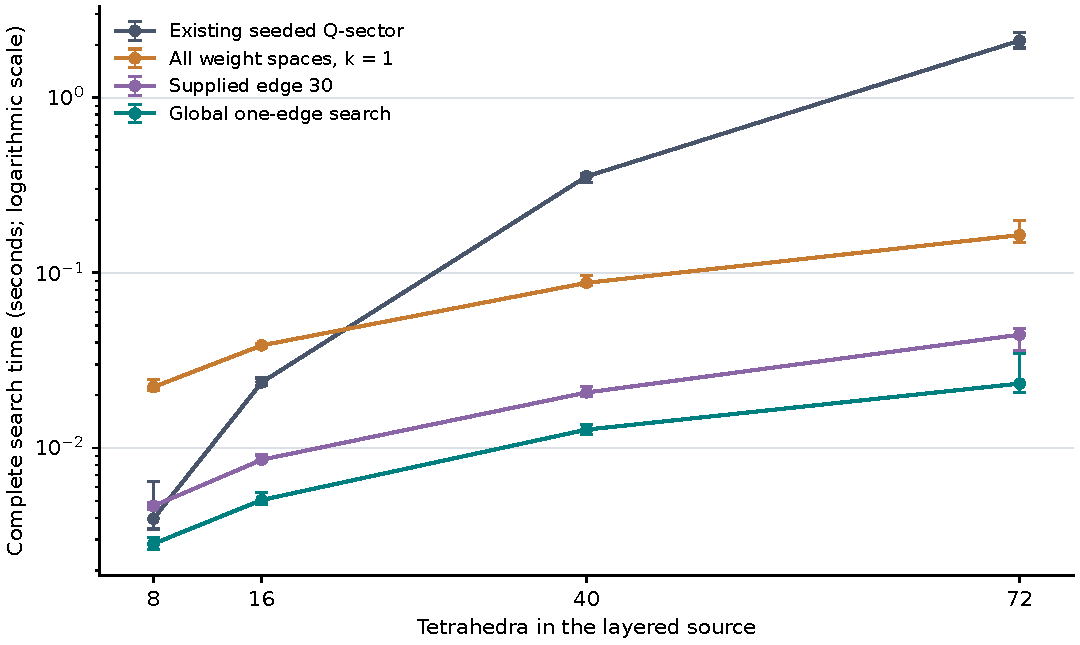
\includegraphics[width=.96\linewidth]{../artifacts/benchmark_plot.pdf}
\caption{Measured medians and full observed ranges on four structured
sources. The vertical axis is logarithmic. The lines connect measurements;
they are not fitted asymptotic laws. Source data and the plotting script
are supplied.}
\label{fig:benchmark}
\end{figure}

The supplied-edge arm includes preparation of its two-dimensional
arrangement, explaining why it is not necessarily faster than the
globally prepared sparse-incidence arm. Coherent-only search completes
quickly but finds no disc, so it is not included as a successful
recognition-time comparator.

On all four labelled fixtures, the global method begins 39 bases,
including the coherent attempt, and makes ten local tetrahedron
reconstructions before its one positive disc query. The deduplicated
global hyperplane counts are 72, 128, 296 and 520. These early-return
counters depend on the serialized edge ordering; the parameter and
completeness statement do not.

The existing seeded sector's matching nullity remains three throughout
the experiment. Its number of kernel variables grows through 16, 40,
112 and 208. The measured difference therefore reflects the amount and
organization of exact algebra and setup, rather than a growing sector
nullity. The elementary new all-subspace method is slower than the
existing solver on the two smallest sources; that unfavorable comparison
is retained. One family and four sizes do not establish a corpus-wide
speedup. The asymptotic theorem comes from the proofs above.

\subsection{Independent and adversarial verification}

The focused edge-discovery suite has 13 tests. It covers rational local
reconstruction, large binary coordinates, dependent coherent columns,
the old and new explicit discs, global caps, cancellation, input
immutability, and replay with corresponding producer functions disabled.

The polynomial vertex gate has seven supplementary tests, including
multiple boundary vertices, rejection of a vertex link with nonzero raw
parity but trivial cohomology class, nonextreme mixed surfaces, determinant
checks against direct small permutation sums, and forged certificates.
At 72 tetrahedra its supported minor has order 216. The compact
certificate has 2,789 bytes, excluding the separately supplied source and
normal vector; exact independent replay succeeds without an orbit query.

Regina independently enumerated 138 standard vertex surfaces across
eight triangulations of one through eight tetrahedra. Exact edge
reconstruction agrees on every vector. Twelve meridians satisfy the
signed/unsigned parity lower bound; eleven applicable subspace searches
recover their targeted standard vertex discs with cancellation support
at most two. The one-edge optimized search also succeeds whenever its
promise applies.

External topology checks confirm the layered family at
$r=0,1,2,4,8$. They are deliberately bounded by 10,000 normal pieces:
Regina's installed documentation states that the connectivity and
orientability methods used expand normal discs, and its compression
test may cut and retriangulate. An initial unrestricted large-family
external audit terminated with exit code 137; no conclusions use its
unretained partial results. The saved record explicitly marks omitted
external checks. Exact native binary certificates and supported-rank
checks remain in force at larger sizes, including the 72-tetrahedron
benchmark witness with more than $3\cdot10^{14}$ normal pieces.

The parallelity supplement's independent audit is described in
Section~\ref{sec:parallelity-interface}; it adds 184 literal geometric
comparisons, including 54 authenticated source comparisons, and huge
binary-coordinate replay. These tests measure different obligations
from vertex-disc discovery and are not added to its sample count.

The maintained suite contains 1,627 collected tests. Successful coverage
was reconciled across the initial broad run (1,512 successful tests) and a
115-test targeted rerun after restoring 20 historical dependency files
from the pinned revision. All 42 initial errors were missing-dependency
or setup errors, with no assertion failures; none remains unresolved.
Both logs, the restored-file list and the complete test identifiers are
included. The 13 new discovery tests are included in the maintained count;
the seven vertex-gate and eleven interface tests are additional.


These are exact-arithmetic programs and human-readable mathematical
proofs with independent review. They are not proof-assistant
formalizations. The principal residual mathematical obligation is the
source-coverage theorem, while the principal remaining implementation
obligations concern optimized general-$k$ enumeration and the transport
of boundary markings through actual geometric replacements.

\subsection{Package and integration procedure}

The archive contains the complete \LaTeX{} sources, compiled PDF,
figures, measurements, certificates, additive source overlay, a patch
against the pinned revision, and reproduction instructions. A small
baseline snapshot includes the dependencies needed by the focused
research experiments; it is not a replacement for the whole repository.

To integrate, first apply the additive discovery files to the pinned
source and run the focused suite. The interface and vertex-gate
supplements can be reviewed independently. Preserve the three trust
boundaries: a certified exterior source, a verified normal surface in
that source, and a justified coverage statement before turning finite
exhaustion into a global negative verdict. Broader default scheduling
should await a mixed-source benchmark that includes unfavorable cases,
relabellings, large-degree edges and preprocessing costs.

\section{A research programme toward quasi-polynomial recognition}
\label{sec:research}

The new parameter moves the main question from discovering all local
quadrilateral choices to controlling the places where geometric and
algebraic intersections disagree. This is useful because a cohomology
generator is inexpensive to compute, and the disagreement is a directly
testable geometric object. The next results should establish control of
that object under certified changes of representation.

\subsection{The structural theorem that would complete this route}

The most direct objective is the following concrete question.

\begin{quote}
Is there an explicit procedure, taking $n^{O(\log n)}$ bit time, which
produces certified polynomial-size exteriors of an $n$-crossing diagram,
such that an unknot has a standard vertex meridian with
$p+|F(D)|\le C\log(n+2)$ in at least one produced source, for an absolute
known constant $C$?
\end{quote}

An affirmative answer combines with Corollary~\ref{cor:qp}; nothing else
in that corollary requires expanding a normal surface. Several aspects
of the wording are essential. The favourable source must be found within
the bound, its relation to the original diagram must be certified, and
vertex potentials count in $p$. A construction with many vertices cannot
silently invoke the one-vertex cancellation theorem. A promising normal
disc that is not a standard vertex disc does not yet meet the promise.

This question is deliberately not elevated to a conjecture that all
sources satisfy. The Whitehead construction rules out that broader
statement. Even the restriction to all one-vertex triangulations remains
an open problem in this investigation and may be false. Constructively
choosing a family of representations is a more flexible target.

\subsection{Geometric questions, in order of dependence}

\begin{enumerate}[label=G\arabic*.]
\item \textbf{Can low cancellation be transferred to a vertex disc?}
Suppose some essential normal disc has cancellation on at most $k$
edges. Is there a standard vertex meridian with at most $f(k)$ such
edges, ideally $f(k)=O(k)$, after a controlled source modification?
The ordinary vertex-disc theorem does not include this support control.
Intersecting a sector with $W_F$ produces extreme rays of the intersection,
which need not be extreme in the full sector. This is exactly the gap a
proof must bridge. A useful first result would identify sufficient
conditions on oriented normal sums under which no cancellation is created
on an edge that was previously coherent.

\item \textbf{Can the Whitehead obstruction persist with one vertex?}
Construct a one-vertex family with $\kappaV=\Omega(t)$, or prove a
quantitative obstruction to collapsing the many interior loop vertices
in Theorem~\ref{thm:whitehead} without destroying the independent
geometric-index barriers. Either result would substantially narrow the
correct global claim. The geometric index of an individual embedded loop
does not by itself control a whole collapsed graph, whose edges may share
vertices and change their isotopy classes.

\item \textbf{How does cancellation behave under certified moves?}
For $2$--$3$, $3$--$2$, boundary layering and crushing operations, derive
local inequalities for the best achievable cancellation support of an
essential disc, while also controlling standard extremality. Boundary
layering has the exact favourable theorem proved here. General Pachner
moves can change the coherent baseline, so comparing only geometric
weights before and after a move is insufficient. A useful move record
should transport the cocycle, candidate disc, affected edge stars and
source correspondence together.

\item \textbf{Can repeated obstacles be removed in batches?}
The Whitehead example has many parallel copies of a single geometric
gadget. Develop a compressed quotient of repeated edge-star regions,
with binary multiplicities and a proof that essential-disc discovery is
preserved. A parameter counting independent gadget types might be small
where literal cancellation support is linear. The hard part is retaining
the ordered attachments and their fibre data; merely aggregating edge
weights can change the embedding problem. The interface operator of
Section~\ref{sec:parallelity-interface} supplies part of the data needed
for a safe batch transformation.

\item \textbf{Can a complexity potential force logarithmic depth?}
Seek a certified simplification or hierarchy move that either exposes a
meridian or decreases a nonnegative structural potential by a fixed
factor. The potential should account for core size, boundary pattern,
vertex-gauge dimension and independent cancellation regions. A decrease
in coordinate weight alone is unsuitable: the layered family has huge
weights but a constant discovery parameter. A decrease in tetrahedron
count alone may fail during useful Pachner exploration. A potential
theorem must bound branching as well as depth.
\end{enumerate}

\subsection{Algebraic and algorithmic questions}

\begin{enumerate}[label=A\arabic*.]
\item \textbf{Implement the general sparse-incidence theorem.}
The highest-confidence next coding task is the row-first enumeration in
Theorem~\ref{thm:incidence}, including its exceptional normalization case.
Use partial injective row-to-edge matchings, incremental exact rank and
canonical descriptions to avoid permutations of the same system.
Completeness should first be compared with the elementary algorithm at
$k=2,3$ on small sources. No heuristic pruning should be credited in the
asymptotic bound without a certificate that it preserves every relevant
invertible system.

\item \textbf{Can the exponent depend on interaction rather than support?}
The determining equations form a hypergraph with row size at most four.
Study dynamic programming over certified decompositions of the affected
edge-star interaction graph. A bag must retain compatible four-point
sectors, rational boundary weight relations and enough global information
to verify a primitive essential disc. Storing only possible total Euler
characteristics would be unsound. The goal is an explicit bound in both
the interaction width and the coefficient bit length, followed by a
geometric theorem controlling that width on selected sources.

\item \textbf{Can algebraic signatures reduce duplicate active systems?}
The present global list has many repeated hyperplanes, and one ray may
have many active descriptions. Investigate reverse search on active
bases or rank certificates indexed by sparse minors. A useful target is
polynomial delay per distinct candidate on a fixed $W_F$. The number of
distinct candidates can still be exponential in the dimension, so such
an output-sensitive result would improve implementation without alone
settling the global complexity question.

\item \textbf{Can the vertex gate replace more expensive positive checks?}
The exact minor and boundary parity certificate is complete for standard
vertex meridians. Measure its crossover with the existing exposed-unit
ray gate and compressed component observer. A sensible schedule first
uses cheap sufficient rank certificates, then the complete supported
rank test when a theoretical vertex-only mode is requested, and reserves
the richer observer for additional restricted rays. Source preparation
and reuse of matrix factors must be included in comparisons.

\item \textbf{How can multiple-vertex sign chambers be compressed?}
The current extension pays $t^{O(p)}$ for the arrangement of cocycle
hyperplanes. Examine whether a certified spanning-tree gauge, boundary
collapses or a small set of relevant vertex potential differences can
reduce $p$ without excluding the unknown disc. Fixing arbitrary vertex
potentials is not harmless: signed intersections of the actual disc may
use a different representative. A valid reduction must transport the
geometric problem, rather than simply delete gauge variables algebraically.
\end{enumerate}

\subsection{Compressed geometry and hierarchy questions}

\begin{enumerate}[label=H\arabic*.]
\item \textbf{Construct the boundary homeomorphisms, not only handle plans.}
For each full or partial disc-base attachment, output the actual collar
maps and transported marked arcs. Prove that disjoint source interfaces
remain disjoint and that the output records their induced order. The
correct relative handle count is already known here; an executable
topological replacement requires more data than that count.

\item \textbf{Convert the result to admissible handles.}
Show that the transported relative additions can be changed to the
uniform-type handle structures required by the hierarchy theory, with
polynomial encoded size. State precisely which boundary patterns are
preserved and which tests establish admissibility. A bounded inherited
core plus interval bundles does not automatically provide this step.

\item \textbf{Extend fibre information beyond separate boundary circles.}
The present signed double cover records transport around each marked
boundary circle. Non-disc bases may require paths connecting distinct
circles and coherent horizontal boundary markings. Identify a finite
set of such paths, bound its size, and certify its relation to the source
charts without expanding the base. Annular and M\"obius examples should
remain explicit regression cases.

\item \textbf{Close the orbit-engine complexity gap.}
The interface theorem has a polynomial reduction to ordinary AHT
counting; the implementation uses weighted traces. Either prove that
these concrete traces and their arithmetic stay polynomial in encoded
source size, or substitute a rigorously bounded counting implementation
for the proof-critical mode. Fast behaviour on long binary multiplicities
is valuable evidence, but does not control every possible interval system.
\end{enumerate}

\subsection{An experimental programme with useful failure criteria}

The next corpus should combine several independently generated classes:
small enumerated solid tori, diagram exteriors with verified provenance,
Pachner walks, layered sources, and sources containing controlled
geometric-index gadgets. For each, record $t$, vertex count, cocycle rank,
the best certified vertex cancellation support found, sector nullity,
maximum coordinate bit length and edge-star degree distribution.
Keep a distinct field for a lower bound or exhaustive result; a heuristic
failure to find a disc is not a lower bound on $\kappaV$.

Compare equal workloads: the same supplied source, the same necessary
preparation, the same certificate acceptance contract, and separately
reported fresh replay. Relabel every source several times to measure
early-return ordering effects. Record failures and cap exhaustion beside
successes. In particular, the elementary all-subspace method's slower
small-source performance should remain visible when evaluating the
optimized replacement.

Three falsifiable milestones would make the next iteration decisive:
\begin{enumerate}
\item General-$k$ row-first enumeration exactly matches elementary
enumeration on a complete small corpus while reducing actual attempted
systems and elapsed time.
\item A certified move family has a proved inequality for cancellation
support or gauge dimension and preserves source size within an explicit
bound. A single verified counterfamily should trigger revision of the
proposed structural claim.
\item Partial disc-base replacements output independently checked
boundary maps and an admissible next handle structure on both the
full-circle and collar fixtures, before being used inside a hierarchy.
\end{enumerate}

\section{Conclusion}

Sparse edge cancellation gives a complete way to discover standard vertex
meridians without first supplying their quadrilateral sector. Its search
spaces have dimension at most $k+1$ in the one-vertex rank-one case, and
sparse equation support gives the sharper explicit enumeration bound.
Exact rank, Euler characteristic and boundary parity suffice to verify
every promised vertex disc in polynomial bit time. The new disc and its
infinite layered extensions demonstrate that this parameter can remain
constant in the presence of dense quadrilateral support, exponential
normal weights and persistent failure of coherent-only discovery.

The Whitehead construction shows why source selection is an essential
part of the proposed global theorem. Ordered parallelity interfaces
provide an additional geometric operation needed for controlled changes
of source, but the admissible replacement and coverage arguments still
require proofs. The precise remaining objective is therefore a
constructive, certified source family with logarithmic $p+k$. Proving it,
or finding the right replacement parameter when it fails, is the central
research task exposed by this continuation.


\begin{thebibliography}{99}
\raggedright
\bibitem{repo} V. Reshetnikov, \emph{ProveIt, Topology/UnknotRecognition},
source revision \path{90e16db798c8d976bbe0c062e07cf20565e0b63a}, inspected
12 October 2026.
\url{https://github.com/VladimirReshetnikov/ProveIt/tree/90e16db798c8d976bbe0c062e07cf20565e0b63a/Topology/UnknotRecognition}.
\bibitem{hlp} J. Hass, J. C. Lagarias and N. Pippenger,
\emph{The computational complexity of knot and link problems},
J. ACM \textbf{46} (1999), 185--211.
\url{https://arxiv.org/abs/math/9807016}.
\bibitem{aht} I. Agol, J. Hass and W. P. Thurston,
\emph{The computational complexity of knot genus and spanning area},
Trans. Amer. Math. Soc. \textbf{358} (2006), 3821--3850.
\url{https://arxiv.org/abs/math/0205057}.
\bibitem{lackenby2026} M. Lackenby,
\emph{Incompressible surfaces, hierarchies and unknot recognition},
arXiv:2607.23350v1, 25 July 2026.
\url{https://arxiv.org/abs/2607.23350}.
\bibitem{slides} M. Lackenby,
\emph{Unknot recognition in quasi-polynomial time}, lecture slides,
February 2021.
\url{https://people.maths.ox.ac.uk/lackenby/quasipolynomial-talk.pdf}.
\bibitem{burton-convert} B. A. Burton,
\emph{Converting between quadrilateral and standard solution sets in
normal surface theory}, Algebraic \& Geometric Topology \textbf{9}
(2009), 2121--2174.
\url{https://arxiv.org/abs/0901.2629}.
\bibitem{burton-complexity} B. A. Burton,
\emph{Computational topology and normal surfaces: theoretical and
experimental complexity bounds}, arXiv:1211.3234v1.
\url{https://arxiv.org/abs/1211.3234}.
\bibitem{geometric-index} K. B. Andrist, D. J. Garity, D. D. Repov\v{s}
and D. G. Wright, \emph{New techniques for computing geometric index},
Mediterranean J. Math. \textbf{14} (2017), article 237.
\url{https://arxiv.org/abs/1711.04267};
\url{https://doi.org/10.1007/s00009-017-1036-1}.
\bibitem{regina} Regina project, \emph{Normal-surface analysis and
calculation-engine documentation}, version 7.4.1 used for independent
experiments.
\url{https://regina-normal.github.io/docs/surfaces-analysis.html}.
\bibitem{parallelity} M. Lackenby,
\emph{The efficient certification of knottedness and Thurston norm},
author manuscript, Theorems 9.2 and 9.3, pp. 72--73.
\url{https://people.maths.ox.ac.uk/lackenby/knp13nov20.pdf}.
\end{thebibliography}
\end{document}
